\documentclass[preprint,12pt,authoryear]{elsarticle}
%% Cognitive Systems Research (Elsevier). Compile with pdfLaTeX + BibTeX (elsarticle-harv).
%% For the final typeset look use: \documentclass[final,3p,times,authoryear]{elsarticle}

\usepackage{amsmath}
\usepackage{amssymb}
\usepackage{booktabs}
\usepackage{graphicx}
\usepackage{multirow}
\usepackage[T1]{fontenc}
\usepackage[utf8]{inputenc}
\usepackage{kotex}          % Korean example sentences (cjk-ko; in TeX Live full / Overleaf)
\usepackage{lineno}
\usepackage[colorlinks=true,linkcolor=blue,citecolor=blue,urlcolor=blue]{hyperref}

\makeatletter
\newcommand{\tablebody}[1]{\@@input #1 }  % primitive input: LaTeX's \input hooks break \bottomrule after the last row
\makeatother
\newcommand{\ko}{\textsc{ko}}
\newcommand{\en}{\textsc{en}}
\newcommand{\de}{\textsc{de}}

\journal{Cognitive Systems Research}

\begin{document}

\begin{frontmatter}

\title{Which Language First? A Pre-Registered Study of Curriculum Order, Forgetting and Recovery in a Recurrent Classifier Constrained by a Fly Central-Brain Connectome}

\author[a]{June woo Kang\corref{cor1}}
\ead{[email]}
\cortext[cor1]{Corresponding author.}
\affiliation[a]{organization={[Department, Institution]},
                city={[City]},
                country={[Country]}}

\begin{abstract}
When one learner acquires the same meaning-judgment task in several languages one after another, does the order matter, how much of the first language is lost while the others are learned, and is it recovered? We report a pre-registered experiment on a recurrent classifier whose recurrent wiring is a fixed 5{,}000-neuron, 524{,}324-connection extract of a \emph{Drosophila} central-brain connectome, with connection strengths learned. English, German and Korean share one controlled template benchmark with four judgment types (roles, negation, spatial relations, quantity). Each seed block trains three monolingual runs, six sequential orders ending in a 1:1:1 review phase, and one mixed baseline. Protocol, code, data, tokenizer and wiring were hash-frozen in a public repository before the main study, the seed count ($N{=}80$) was chosen by pre-simulation, and two contrasts were pre-specified. An operator-scheduled stop ended the study at 753 of 800 runs; we analyse the longest complete prefix of the pre-registered seed order (75 blocks) under a rule declared before any outcome was read. Korean-first orders reached three-language mastery with 112{,}230 fewer training examples than Korean-last orders (about 26\%; Holm-adjusted $p{=}2.7{\times}10^{-17}$), and orders keeping English and German adjacent needed 39{,}151 fewer examples than orders separating them (about 9\%; $p{=}4.6{\times}10^{-8}$). Descriptively, the order effect tracks which language is mastered within the cap-limited first stage, where the quantity judgment is the bottleneck in every language. The first language fell to near chance while the others were trained and recovered in review in all 450 sequential runs; mixed training was costlier than every sequential order; mastery generalised to held-out items within the training sentence frame but not to unseen outer frames. Conclusions are conditional on the frozen items, input representation, model and policy; we claim neither universal language difficulty nor, having run no control wiring, any effect specific to the fly connectome.
\end{abstract}

\begin{highlights}
\item Pre-registered curriculum-order study on a fly-connectome recurrent classifier
\item Korean-first orders needed 26\% fewer examples than Korean-last orders (75 seeds)
\item The order effect tracks which language is mastered in the cap-limited first stage
\item The first language drops to chance in later stages and fully recovers in review
\item Mastery generalises within the sentence frame but not to unseen outer frames
\end{highlights}

\begin{keyword}
continual learning \sep catastrophic forgetting \sep curriculum order \sep multilingual learning \sep connectome-constrained network \sep pre-registration
\end{keyword}

\end{frontmatter}

\linenumbers


\section{Introduction}

Sequential multilingual learning raises a question that appears both in human second-language research and in continual learning: when the same learner must acquire several languages one after another, does the order change the total cost, and what happens to the language learned first while the others are being learned? Controlled answers are rare because the natural setting confounds order with age, exposure, motivation and typological distance, and because machine-learning studies of curriculum order typically report a handful of seeds without a pre-specified analysis.

This paper reports one controlled, pre-registered measurement. The learner is a recurrent classifier whose recurrent structure is fixed to a real central-brain connectome of the fruit fly (5{,}000 neurons, 524{,}324 directed connections) and whose connection strengths, biases, leak rates and small input/output adapters are trained. The task is the same in all three languages: decide whether two sentences express the same proposition, over four judgment types (thematic roles, negation, spatial relations, quantity). Stimuli are generated from one template grammar rendered into English, German and Korean, so that the three languages share meanings, foils and splits exactly. Every seed block trains ten runs from scratch: three monolingual runs, six sequential orders that end with a 1:1:1 review phase, and a mixed 1:1:1 baseline.

We started from a public repository \citep{flygpt} that reports a small early-training advantage of connectome-derived wiring over matched random wiring and no detectable difference at the end of training. We audited those claims rather than assuming them (Appendix~\ref{app:wiring}) and re-posed the problem as a measurement problem: with the wiring held fixed, what is the cost, in training examples, of reaching a common mastery criterion under each curriculum? Our contributions are the following, and we state them only to the extent that the evidence supports them.

\begin{enumerate}
\item A protocol frozen by hash in a public repository before the main study, a seed count chosen by pre-simulation against explicit power and family-wise error criteria, and a complete public record of every technical failure and every procedural amendment, including the deviation that ended the study at 753 of 800 runs (Sections~\ref{sec:design} and~\ref{sec:execution}).
\item Two pre-specified contrasts, both significant after Holm adjustment with interval estimates that exclude zero: Korean-first orders were about 26\% cheaper than Korean-last orders, and orders with English and German adjacent were about 9\% cheaper than orders separating them (Section~\ref{sec:contrasts}).
\item A descriptive decomposition showing that the order effect tracks the attainment of the cap-limited first stage, which in turn matches the monolingual attainment of each language and the same bottleneck judgment type (Section~\ref{sec:decomposition}).
\item Seventy-five-seed forgetting and recovery curves (Section~\ref{sec:forgetting}), an independent held-out test of terminal checkpoints, and a negative result on transfer to held-out outer sentence frames (Section~\ref{sec:test}).
\end{enumerate}

Three things we do \emph{not} claim. We do not claim that any language is universally easier or harder: the German items in this benchmark were mastered less often within the cap, and that is a statement about these items, this tokenizer and this model. We do not claim any effect specific to the fly connectome: the main study used only the real wiring, and a degree-preserving shuffled control that was budgeted was never run. We do not report or interpret the fifteen pairwise order comparisons; the two pre-specified contrasts are the only confirmatory results.

\section{Related work}

\paragraph{Catastrophic forgetting and rehearsal.} That sequentially trained connectionist networks overwrite earlier tasks has been known since \citet{mccloskey1989} and \citet{ratcliff1990}; \citet{french1999} and \citet{parisi2019} review the phenomenon and the remedies, of which interleaved rehearsal \citep{robins1995} is the closest to the review phase used here. Regularisation approaches such as elastic weight consolidation \citep{kirkpatrick2017} are not used: our aim is to measure forgetting and recovery under a fixed, simple policy, not to prevent it.

\paragraph{Curriculum and language order.} Curriculum learning \citep{bengio2009} studies the order of examples within one task. Cross-lingual transfer in multilingual models depends on the source language and on typological and lexical distance \citep{pires2019,lin2019,conneau2020}, but those studies compare languages that differ in corpus size, script and pre-training exposure. Here the three languages share one meaning inventory, one foil construction and one tokenizer budget, so that order effects cannot be attributed to differences in content.

\paragraph{Connectome-constrained models.} Reservoir computing trains a readout on a fixed random recurrent network \citep{jaeger2001,maass2002}. Connectome-constrained models replace the random structure with measured wiring; \citet{lappalainen2024} showed that a network constrained by the fly visual-system connectome predicts neural responses after task training. Dense connectomes of the fly central brain \citep{scheffer2020} and of the whole brain \citep{dorkenwald2024} are now available. The wiring used here is a 5{,}000-neuron dense-core extract of the MaleCNS central-brain connectome \citep{berg2026malecns} published with an open-source language model \citep{flygpt}; we use it as a fixed sparse structure with learned strengths and make no claim that this structure is necessary for our results.

\paragraph{Pre-registration and statistical practice in ML.} Sensitivity of deep-learning results to seeds and analysis choices is well documented \citep{henderson2018,bouthillier2019,agarwal2021}, as is the need for corrected significance testing in NLP evaluation \citep{dror2018}. Pre-registration separates confirmatory from exploratory claims \citep{nosek2018}, and sample-size justification by simulation is standard in other empirical sciences \citep{lakens2022}. We follow those practices, including a pre-specified restricted-mean cost measure adapted from survival analysis \citep{royston2013}.

\section{Task and stimuli}
\label{sec:task}

\subsection{Judgment task}

Each item is a pair of sentences in one language. The label is 1 if the propositions expressed by the two sentences mutually entail each other and 0 otherwise. The second sentence is always a syntactically inverted rendering of the same scene (passive voice or argument reordering, as available in each language), so that surface overlap does not reveal the label. Four judgment types are generated from one scene grammar over 12 animal nouns, 6 colours and 4 attribute adjectives (288 entity descriptions), 3 transitive verbs, 3 spatial axes and 7 number words:

\begin{itemize}
\item \textbf{Roles.} Two coordinated clauses with the same two entities in exchanged roles and two different verbs; the foil exchanges the verbs.
\item \textbf{Negation.} Two coordinated clauses with exchanged roles and opposite polarity; the foil flips which clause is negated.
\item \textbf{Spatial relations.} Two coordinated clauses about two entity pairs on one axis (left/right, above/below, front/behind); the foil reverses the direction. The task definition stipulates one fixed external viewer for horizontal terms and gravity for vertical terms, so that converse relations (\emph{A is left of B} $\Leftrightarrow$ \emph{B is right of A}) hold in all three languages (Appendix~\ref{app:stimuli}).
\item \textbf{Quantity.} Two counted noun phrases; the foil exchanges the two counts, so that true and false items contain the same bag of number words.
\end{itemize}

Table~\ref{tab:examples} gives one item per language. In German the inverted sentence uses the passive with a dative agent phrase, and subordinate frames use verb-final order; in Korean the inversion scrambles object and subject, and the two coordinated clauses are nominalised identically (\ldots다는 것과 \ldots다는 것이 모두 사실이다) so that connective inflection cannot reveal which clause is negated.

\begin{table}[t]
\caption{One \emph{roles} item per language (label 1, mutual entailment). Sentence B is the inverted rendering of the same scene; the foil (label 0) exchanges the two verbs.}
\label{tab:examples}
\centering
\small
\begin{tabular}{lp{0.85\linewidth}}
\toprule
\en\ A & The small red dog sees the young blue cat and the young blue cat greets the small red dog. \\
\en\ B & The young blue cat is seen by the small red dog and the small red dog is greeted by the young blue cat. \\
\midrule
\de\ A & Der kleine rote Hund sieht die junge blaue Katze und die junge blaue Katze grüßt den kleinen roten Hund. \\
\de\ B & Die junge blaue Katze wird von dem kleinen roten Hund gesehen und der kleine rote Hund wird von der jungen blauen Katze gegrüßt. \\
\midrule
\ko\ A & 작은 빨간색 개가 어린 파란색 고양이를 본다는 것과 어린 파란색 고양이가 작은 빨간색 개를 반긴다는 것이 모두 사실이다. \\
\ko\ B & 어린 파란색 고양이를 작은 빨간색 개가 본다는 것과 작은 빨간색 개를 어린 파란색 고양이가 반긴다는 것이 모두 사실이다. \\
\bottomrule
\end{tabular}
\end{table}

\subsection{Stimulus generation and splits}

A scene is drawn, hashed to a \emph{semantic orbit} (the set of items that differ only by exchanging entities, counts, polarity or direction), and the orbit, not the item, is assigned to a split. Foils and all three translations of an item therefore live in the same split, and no evaluation item shares an orbit with a training item. The training split has 5{,}000 items per language and judgment type (60{,}000 unique items per run); two development panels (A and B) hold 1{,}000 items per cell (language $\times$ type, twelve cells) and are scored alternately; an independent test split was generated from fresh orbits after all exploratory work, checked for zero overlap with every earlier dataset, and applied exactly once to each run's terminal checkpoint. Evaluation items are rendered in the same declarative frame as training (the \emph{primary} rendering, used for all mastery decisions). The same held-out items are also rendered in a held-out outer frame (a truth question, a reported clause, or a conditional, one family per split); these \emph{auxiliary} renderings are scored only on terminal checkpoints and never enter mastery decisions.

\subsection{Input representation}

Sentences are tokenised with one shared byte-level byte-pair encoding (BPE; \citealp{sennrich2016}, applied to bytes as in \citealp{radford2019}) trained on the three-language training split with merges forbidden across whitespace; the requested vocabulary of 4{,}096 saturated at 832 types, which we kept rather than padding. Encoded sentence pairs (two sentences with a separator and an end token) are 26--58 tokens long in the training split, with language means of 43.1 (English), 41.8 (German) and 38.0 (Korean). The choice of a word-bounded tokenizer was made after an exploratory diagnostic showed that a whole-string BPE fused content words with frame words, so that 68--77\% of tokens in outer-frame evaluation sentences had never been seen in training (Appendix~\ref{app:history}).

\subsection{Stimulus review}
\label{sec:review}

Generation is not validation. The benchmark was reviewed by a language model (Claude) under a written procedure: a 600-item audit sample (200 per language) was judged for label correctness and fluency by independent sessions, and a 21-row checklist covered grammatical phenomena in the primary and auxiliary renderings. A first round flagged 24 checklist rows (for example a Korean topic particle inside the spatial frame, a German dative article form, and a colour adjective), which led to template revision v4.6. A second round on the revised benchmark reached perfect item agreement with the reference labels in all three languages ($\kappa{=}1.0$, no fluency failures) but raised three checklist flags, each from a single session. Under the original rule any flag blocked certification. Rather than iterate indefinitely, we amended the rule before the main study: each flag was adjudicated in a fresh session, and only flags that could change a reference label were treated as blocking. One was: the spatial-relation definition had not fixed a reference frame. We resolved it by stipulating the frame (no sentence or label changed) and re-judging the 150 spatial audit items under the stipulation (150/150 agreement). The two non-blocking flags constrain interpretation (Section~\ref{sec:limitations}). No native speaker reviewed the stimuli; this is a limitation of the benchmark, not of the analysis.

\section{Model and training policy}
\label{sec:model}

\subsection{Network}

The recurrent core is a graph of $n{=}5{,}000$ scalar neurons and $E{=}524{,}324$ directed connections: a dense-core extract of the central brain of the MaleCNS v1.0 connectome \citep{berg2026malecns,hartford2026malecns}, distributed with an open-source language model \citep{flygpt}. The graph, its provenance and its hash were frozen. Of the neurons, 256 receive input and 512 are read out. Each token $x_t$ is embedded ($d{=}32$) and projected by a linear adapter onto the input neurons to form a drive $u_t\in\mathbb{R}^n$ (zero on non-input neurons). The state $h\in\mathbb{R}^n$ is updated twice per token (\emph{microsteps} $=2$):
\begin{equation}
h \leftarrow (1-\lambda)\odot h + \lambda\odot\tanh\!\left(W h + u_t + b\right),
\qquad W_{ji} = \frac{w_{ji}}{\sqrt{\mathrm{indeg}(j)}}\ \text{for } (i\!\to\! j)\in E,
\end{equation}
where the connection strengths $w$, the biases $b$ and the leak rates $\lambda{=}\sigma(\ell)$ are trained and the sparsity pattern of $W$ is fixed. The state after the last token of the pair, restricted to the 512 output neurons, feeds a linear layer with two logits. Trainable parameters total 570{,}422 (524{,}324 strengths, 5{,}000 biases, 5{,}000 leaks, 26{,}624 embedding, 8{,}448 input adapter, 1{,}026 head). The sparse recurrence runs in a custom CUDA kernel whose equivalence to a dense reference implementation was verified on 48 comparisons before the freeze.

Optimisation uses AdamW \citep{loshchilov2019} with learning rate $3{\times}10^{-4}$ for the recurrent parameters and $10^{-3}$ for the adapters, weight decay $0.01$, gradient clipping at $1.0$ and an effective batch of 256 sentence pairs. Nothing is pre-trained; every run starts from a seeded random initialisation of the strengths and adapters.

\subsection{Curricula, evaluation and mastery}

Every 5{,}120 training examples the run scores a full panel: 1{,}000 items for each of the twelve cells (development panels A and B alternate). A cell is \emph{mastered} when its accuracy is at least 0.8 on two consecutive scheduled panels. Three policies share this evaluation:

\begin{itemize}
\item \textbf{Monolingual.} One language, four cells; stops when all four are mastered or at 200{,}000 examples (\emph{administrative cap}).
\item \textbf{Sequential.} Three stages in a fixed order. A stage ends when the current language's four cells are mastered or at 200{,}000 examples of that stage (\emph{stage cap}, recorded as such). Model and optimiser state carry over. After the third stage the run trains on a 1:1:1 mixture of the three languages (\emph{review}) until all twelve cells are mastered or the total reaches 900{,}000 examples.
\item \textbf{Mixed.} A 1:1:1 mixture from the start with the same evaluation and stopping rules (cap 900{,}000).
\end{itemize}

The six sequential orders are \en-\de-\ko, \en-\ko-\de, \de-\en-\ko, \de-\ko-\en, \ko-\en-\de and \ko-\de-\en. One seed block is the ten runs (three monolingual, six sequential, one mixed) sharing a seed; the seed fixes initialisation and data order. Because the first stage of a sequential run depends only on the seed and the first language, the two orders that share a first language share their first stage exactly.

\subsection{Outcome measures}

The primary outcome of a sequential or mixed run is the number of training examples at which all twelve cells were confirmed mastered; a run that reaches the cap contributes the cap (restricted cost). The pre-specified summary of an order is the restricted mean cost over seeds. Monolingual runs contribute the same quantity per cell and per language with cap 200{,}000. The independent test split is scored once on the terminal checkpoint of every run, and the auxiliary outer-frame renderings are scored there as well. Confirmed mastery is a within-run decision rule; the independent test is the only evaluation on data never used for any decision.

\section{Pre-registered design}
\label{sec:design}

\subsection{Confirmatory contrasts and inference}

Let $c_{s,o}$ be the restricted cost of order $o$ in seed block $s$. Two contrasts were pre-specified:
\begin{align}
\Delta_{\mathrm{KO}} &= \tfrac{1}{2}\left(c_{\en\de\ko}+c_{\de\en\ko}\right)-\tfrac{1}{2}\left(c_{\ko\en\de}+c_{\ko\de\en}\right), \\
\Delta_{\mathrm{adj}} &= \tfrac{1}{4}\left(c_{\en\de\ko}+c_{\de\en\ko}+c_{\ko\en\de}+c_{\ko\de\en}\right)-\tfrac{1}{2}\left(c_{\en\ko\de}+c_{\de\ko\en}\right),
\end{align}
the first comparing Korean-last with Korean-first orders and the second comparing orders in which English and German are adjacent with the two orders in which Korean separates them. Each contrast is computed within seed block and tested with a two-sided paired $t$-test; the two $p$-values are Holm-adjusted \citep{holm1979} at family level $0.05$. Interval estimates are 97.5\% $t$-intervals (Bonferroni coverage for the two contrasts) and, as a sensitivity check, 95\% percentile intervals from 10{,}000 seed-block bootstrap resamples with a fixed seed. Restricted means per order are reported with descriptive intervals. The fifteen pairwise comparisons among orders are not tested.

\subsection{Sample size by simulation}
\label{sec:samplesize}

The seed count was chosen before the main study from a pre-registered procedure. Fifteen pilot blocks (150 runs, seeds disjoint from the main study) supplied a dispersion bound (bootstrap 97.5\% coefficient of variation of the order costs, inflated by 25\%: 0.419) and a censoring bound (0.181). A simulation grid then generated restricted costs from log-normal and Weibull families at coefficients of variation up to the pilot bound, censoring up to the grid ceiling, and zero latent correlation between orders (the most conservative value consistent with the pilot), for a target effect of 20\% of the reference mean. The approval rule required a Monte Carlo lower bound on power of at least 0.8 for both contrasts and an upper bound on the null family-wise error rate of at most 0.06 across all null scenarios. Table~\ref{tab:design} shows the outcome for each candidate $N$: the smallest passing $N$ was 60, and the rule selects the largest passing $N$ within the reserved budget, which was $N{=}80$ (power lower bound 0.929; family-wise error upper bound 0.0538; 327 GPU-hours extrapolated from per-run upper bounds, reserved with 25\% contingency as 409 hours). The evaluation interval of 5{,}120 was retained because re-reading the pilot logs on coarser grids distorted between-language cost differences by 3.1\% at 10{,}240 and 9.3\% at 20{,}480.

\begin{table}[t]
\caption{Pre-simulation table used to choose $N$ (frozen before the main study). Power lower bound and null family-wise error upper bound are Monte Carlo bounds over the stress envelope; GPU and calendar hours are extrapolated upper bounds.}
\label{tab:design}
\centering
\small
\begin{tabular}{rrrrr}
\toprule
$N$ & Power (lower) & Null FWER (upper) & GPU h & Calendar h \\
\midrule
\tablebody{tables/design.tex}
\bottomrule
\end{tabular}
\end{table}

\subsection{Freeze and execution rules}

Before launch, the protocol file, the analysis code, the dataset, the tokenizer and the wiring were hashed, the 800-run manifest (seeds 30001--30080 in a fixed order) was written, and the commit was pushed to a public repository. Execution rules were fixed as well: a technical failure is recorded, charged to a ledger and repeated from scratch or resumed from its last checkpoint under a new reservation, and no seed block may be excluded or selected on the basis of outcomes; no contrast is computed before the study is complete; a run that never masters contributes its cap. All analysis code paths that summarise contrasts refuse to run unless every pre-registered block is present.

\subsection{Amendments recorded before the main study}
\label{sec:amendments}

Two procedural amendments were made after seeing intermediate results but before any main-study run, and are recorded with their timing and reasons. First, the review certification rule was amended as described in Section~\ref{sec:review}. Second, the family-wise error criterion was initially evaluated with 5{,}000 Monte Carlo repetitions per null scenario; the resulting Wilson upper bounds (0.060--0.064) exceeded the 0.06 threshold by an amount within Monte Carlo error, so the bound and the threshold were kept and the repetitions were fixed at 50{,}000 for one further run with fresh seeds, after which the largest upper bound was 0.0554 and all $N\ge 60$ passed. Neither amendment changed thresholds, caps, tasks or the contrast definitions; neither is described as pre-registered from the start.

\section{Results}
\label{sec:results}

\subsection{Execution and deviation from the pre-registered $N$}
\label{sec:execution}

The main study launched at 15:56 UTC on the freeze day and ran on two consumer GPUs, then on one after the second GPU failed twice (Appendix~\ref{app:execution}). Six technical failures occurred (a start-up race on a shared audit file, two GPU bus failures, one failed resume from a two-device checkpoint on one device, one transient memory error, one server reboot); every failure was recorded, charged and recovered by repeating or resuming the run, and no block was excluded. An operator-scheduled stop, ordered for reasons external to the study, ended the campaign after 5.3 days with 753 of 800 runs complete; the run active at that moment had reached its cap six seconds earlier, so no run was interrupted. The operator then decided not to resume.

The frozen analysis code refuses this state (``incomplete blocks''), and we did not modify it. Instead we declared one rule, before reading any outcome: the analysis set is the longest prefix of the pre-registered seed order whose blocks are complete. That prefix is seeds 30001--30075 (750 runs); block 30076 had only its three monolingual runs and was excluded; blocks 30077--30080 were never started. The pre-registered summary was then applied unchanged to the prefix. The power and family-wise error guarantees were computed for $N{=}80$; at $N{=}75$ we can only bracket them by the frozen table (power lower bound 0.887 at $N{=}70$ and 0.929 at $N{=}80$; family-wise error upper bound 0.054 at both). The deviation is a consequence of the stop, not of the data, and we did not compute a post-hoc power value for $N{=}75$.

\subsection{Confirmatory contrasts}
\label{sec:contrasts}

Table~\ref{tab:contrasts} reports the two pre-specified contrasts and Table~\ref{tab:rmst} the restricted mean cost of each order and of the mixed baseline (Figure~\ref{fig:rmst}). All 450 sequential runs and 74 of 75 mixed runs reached three-language mastery within the 900{,}000-example cap. Korean-last orders cost 112{,}230 more examples than Korean-first orders (437{,}692 versus 325{,}461 on average, about 26\%), and orders separating English and German by Korean cost 39{,}151 more than orders keeping them adjacent (420{,}727 versus 381{,}577, about 9\%). Both Holm-adjusted $p$-values are far below 0.05, and both the simultaneous $t$-intervals and the bootstrap intervals exclude zero. These two statements are the confirmatory results of the study; everything that follows is descriptive.

\begin{table}[t]
\caption{Pre-specified contrasts, $N{=}75$ seed blocks. Differences in training examples; positive means the first-named group is costlier. $p$-values are Holm-adjusted; the simultaneous interval is a 97.5\% paired $t$-interval; the bootstrap interval is a 95\% percentile interval over 10{,}000 seed-block resamples.}
\label{tab:contrasts}
\centering
\small
\resizebox{\linewidth}{!}{%
\begin{tabular}{lrrll}
\toprule
Contrast & Difference & Holm $p$ & Simultaneous CI & Bootstrap CI \\
\midrule
\tablebody{tables/contrasts.tex}
\bottomrule
\end{tabular}}
\end{table}

\begin{table}[t]
\caption{Restricted mean cost to confirmed mastery of all twelve cells (cap 900{,}000), $N{=}75$. The 95\% $t$-interval is descriptive. Events: runs that mastered before the cap.}
\label{tab:rmst}
\centering
\small
\begin{tabular}{lrlrr}
\toprule
Condition & RMST & 95\% $t$-CI & SD & Events \\
\midrule
\tablebody{tables/rmst.tex}
\bottomrule
\end{tabular}
\end{table}

\begin{figure}[t]
\centering
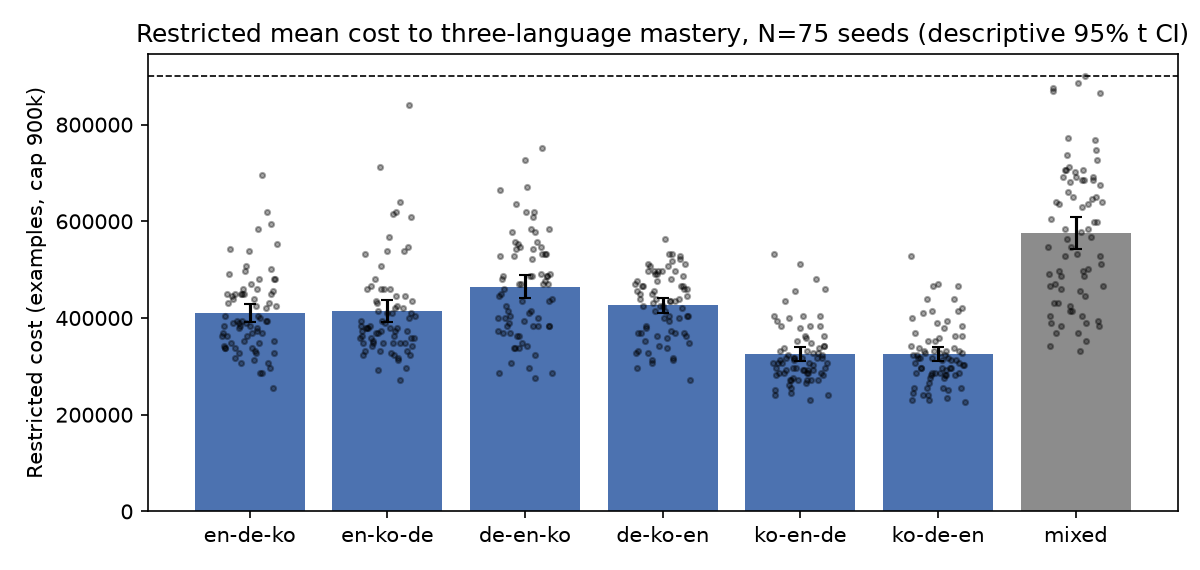
\includegraphics[width=0.85\linewidth]{figures/rmst-by-order.png}
\caption{Restricted mean cost to three-language mastery by condition (bars), with each of the 75 seed blocks as a point and descriptive 95\% $t$-intervals. The dashed line is the 900{,}000-example cap.}
\label{fig:rmst}
\end{figure}

\subsection{Decomposition: what the first stage attains}
\label{sec:decomposition}

Table~\ref{tab:stages} shows, for each order, how many first, second and third stages ended in mastery versus at the 200{,}000-example stage cap, together with the mean stage length and the mean length of the review phase. The first stage is the only one that regularly hits its cap: German was mastered in 12 of 75 first stages, English in 40 of 75 and Korean in 57 of 75. Second and third stages were almost always mastered, and quickly (mean 43{,}000--116{,}000 examples). Review lengths were shortest for Korean-first orders (34{,}000--36{,}000) and longest for German-first orders (66{,}000--73{,}000). The mean cost of an order is therefore, to a first approximation, a cap-limited first stage plus two short transfer stages plus a review whose length depends on how much of the first language must be recovered and how much of the first stage was left unlearned.

\begin{table}[t]
\caption{Sequential stages by order, $N{=}75$: language, runs mastered/runs ending at the stage cap, and mean stage length in examples; final column is the mean review length. The two orders sharing a first language share their first stage exactly.}
\label{tab:stages}
\centering
\small
\resizebox{\linewidth}{!}{%
\begin{tabular}{lllll}
\toprule
Order & Stage 1 & Stage 2 & Stage 3 & Review \\
\midrule
\tablebody{tables/stages.tex}
\bottomrule
\end{tabular}}
\end{table}

The same ranking appears in the monolingual runs (Table~\ref{tab:mono}), which train one language with the same 200{,}000-example cap: within it, Korean mastered all four cells in 59 of 75 runs, English in 47 and German in 14. In every language the \emph{quantity} judgment was the bottleneck: it was left unmastered in 27 English, 61 German and 12 Korean runs, while roles and negation were mastered in nearly every English and Korean run. We read the two pre-specified contrasts in this light. Placing Korean first fills the cap-limited stage with the language whose items this model learns fastest and defers the slower languages to stages where transfer makes them fast; placing German first spends the cap on the language least often mastered within it and then has to recover it in review. Separating English and German by Korean adds a Korean stage between two languages whose items, in this benchmark, share templates and word order more closely. This is a descriptive account consistent with the data, not a mediation analysis.

\begin{table}[t]
\caption{Monolingual attainment, cap 200{,}000, $N{=}75$ per language. Restricted mean cost to confirmed mastery per cell and for all four cells; ``censored'' counts runs that reached the cap without mastering the cell.}
\label{tab:mono}
\centering
\small
\begin{tabular}{lrlrr}
\toprule
Cell & RMST & 95\% $t$-CI & Median & Censored \\
\midrule
\tablebody{tables/mono.tex}
\bottomrule
\end{tabular}
\end{table}

\subsection{Forgetting and recovery}
\label{sec:forgetting}

We define a language's accuracy at a scheduled panel as the mean of its four cells. For each sequential run and each of its first two stages we record the accuracy at the last panel before the stage ended, the minimum over all later panels, the accuracy at the last panel before the review phase, and the accuracy at the run's end (Table~\ref{tab:forgetting}, Figure~\ref{fig:forgetting}). While the other languages were trained, the first language fell from 0.92--0.94 (English, Korean) to a minimum of 0.50--0.62, that is, to or near chance, and was still at 0.55--0.64 when review began. In the review phase it was recovered in every one of the 450 sequential runs, by our single-panel criterion (all four cells $\ge 0.8$) after a mean of 26{,}000--31{,}000 examples for English- and Korean-first orders. German-first orders behave differently: German left its first stage at 0.70 on average, mostly unmastered, so its subsequent decline is less forgetting than incomplete learning, and its recovery took 60{,}000--65{,}000 examples. The second language shows the same pattern with a smaller drop (minimum 0.57--0.70) and a faster recovery (9{,}000--24{,}000 examples).

\begin{table}[t]
\caption{Forgetting and recovery of the first- and second-stage language, $N{=}75$ per order. Accuracies are means over runs of the language's mean cell accuracy at the stage end, at its minimum afterwards, at the start of review and at the run's end. ``Recovered'' counts runs with all four cells $\ge 0.8$ on some panel after review start; ``recovery'' is the mean number of review examples to that panel; the last column counts runs whose confirmed mastery of the language was recorded only in review.}
\label{tab:forgetting}
\centering
\scriptsize
\resizebox{\linewidth}{!}{%
\begin{tabular}{llrrrrrrr}
\toprule
Order & Language & Stage end & Minimum & Review start & Run end & Recovered & Recovery & Confirmed in review \\
\midrule
\tablebody{tables/forgetting.tex}
\bottomrule
\end{tabular}}
\end{table}

\begin{figure}[t]
\centering
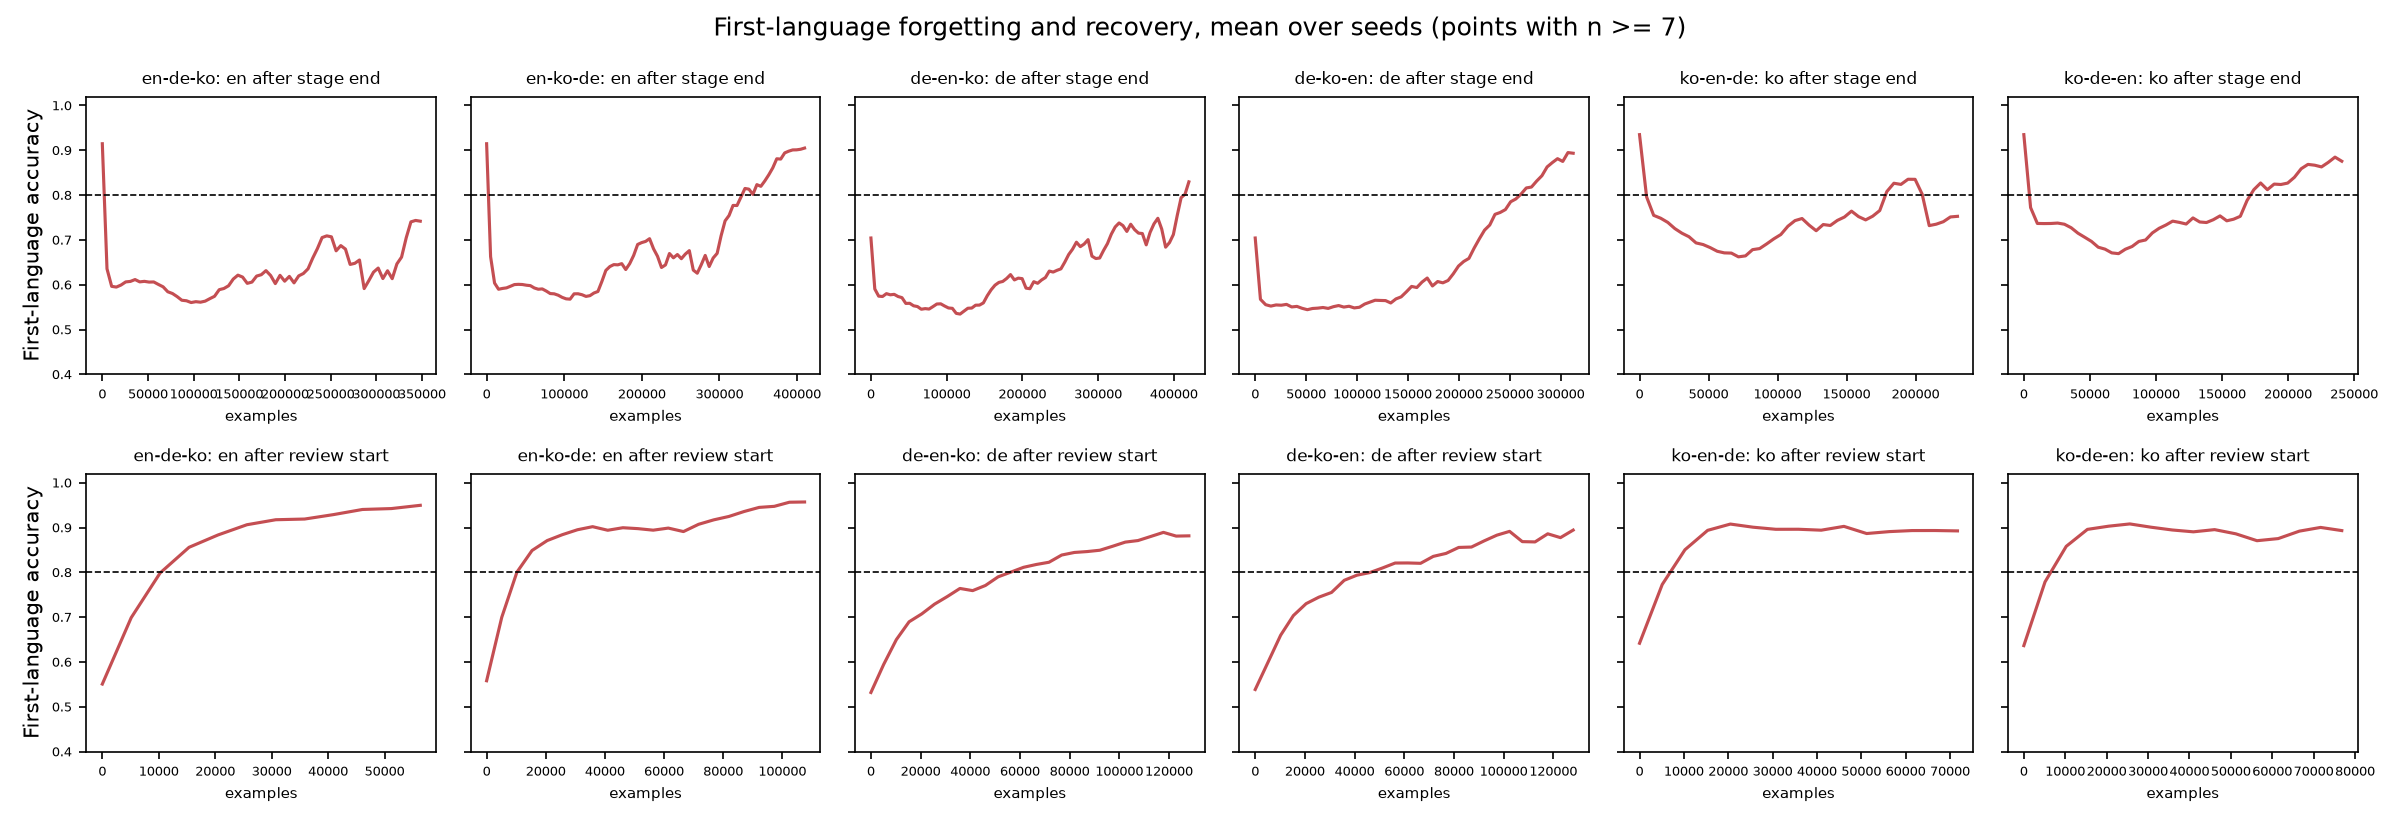
\includegraphics[width=\linewidth]{figures/forgetting-recovery-first-language.png}
\caption{First-language accuracy (mean of four cells) averaged over seeds, aligned to the end of its stage (top) and to the start of the review phase (bottom), for each order. Only points averaging at least seven runs are drawn; late points average the slower runs still training.}
\label{fig:forgetting}
\end{figure}

\subsection{Mixed baseline}

Training on the 1:1:1 mixture from the start was costlier than every sequential order (restricted mean 575{,}814 versus 325{,}086--464{,}828; Table~\ref{tab:rmst}), and one mixed run reached the 900{,}000 cap without confirming any language. This comparison was not pre-specified and we report it descriptively. Per-language confirmed mastery in the mixed runs occurred at 522{,}000--567{,}000 examples on average (Appendix~\ref{app:extra}), consistent with the three languages competing for the same budget rather than transferring to one another as they do across sequential stages.

\subsection{Independent test and outer-frame transfer}
\label{sec:test}

Table~\ref{tab:test} summarises the independent test split scored on terminal checkpoints (full cell table in Appendix~\ref{app:extra}; Figure~\ref{fig:test}). In all sequential and mixed conditions every one of the twelve cells averaged at least 0.85, and at least 96\% of runs scored at least 0.8 in every cell; the quantity cells were lowest (0.85--0.92). Monolingual German checkpoints, mostly unmastered at the cap, scored 0.62--0.75. Mastery as defined by the within-run panels therefore generalises to held-out meanings within the training sentence frame.

It does not generalise to held-out outer frames. The auxiliary renderings of the same test items (conditional frame) and of the development panels (truth question, reported clause) scored 0.33--0.55 in every condition and cell, that is, at or below chance. Several cells are systematically below 0.5 (for example English negation under the truth-question frame, 0.33--0.42), which indicates a consistent response bias under the unseen frame rather than partial transfer. We did not test this bias further; the auxiliary panels were pre-specified as transfer indicators only.

\begin{table}[t]
\caption{Independent test on terminal checkpoints, $N{=}75$ per condition: mean accuracy over the four cells of each language (minimum cell in parentheses), and the range of the outer-frame auxiliary scores across the three auxiliary panels and all cells.}
\label{tab:test}
\centering
\small
\resizebox{\linewidth}{!}{%
\begin{tabular}{lllll}
\toprule
Condition & \en\ mean (min) & \de\ mean (min) & \ko\ mean (min) & Outer-frame range \\
\midrule
\tablebody{tables/test_lang.tex}
\bottomrule
\end{tabular}}
\end{table}

\begin{figure}[t]
\centering
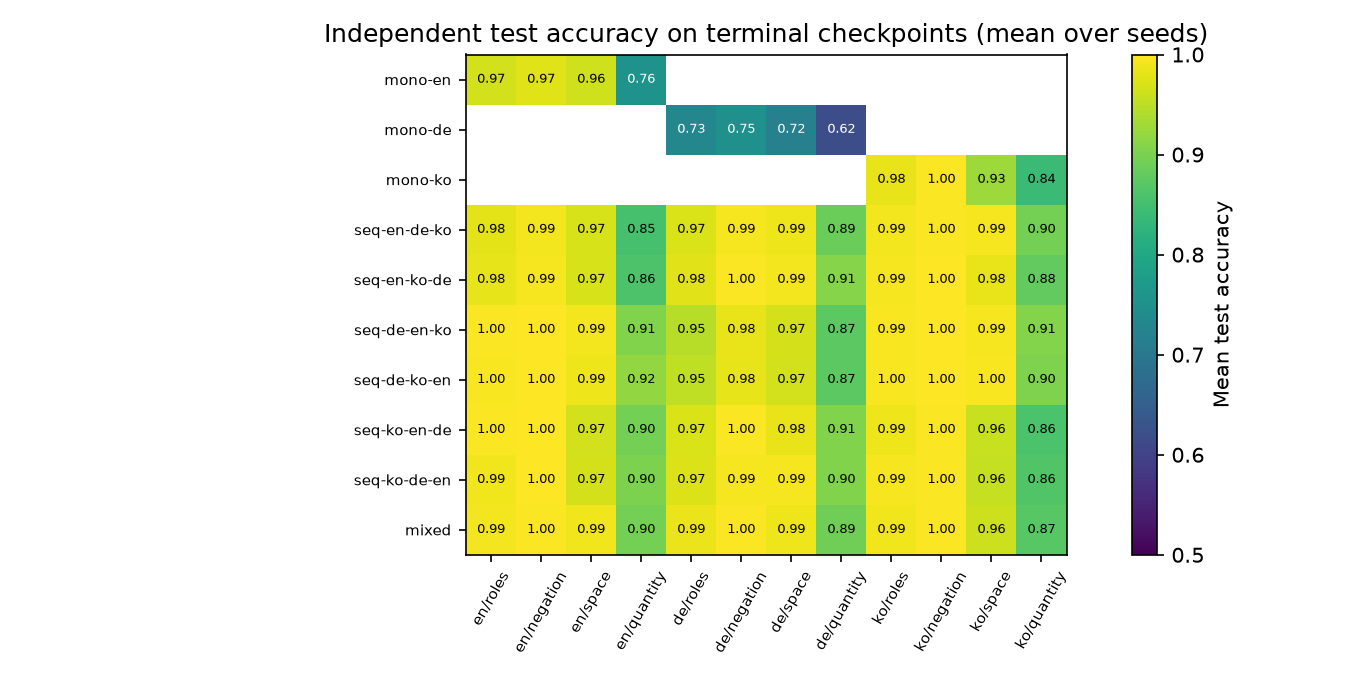
\includegraphics[width=0.8\linewidth]{figures/independent-test.png}
\caption{Independent test accuracy on terminal checkpoints, mean over seeds, by condition and cell.}
\label{fig:test}
\end{figure}

\subsection{Cost}

The 753 completed runs used 68.4 GPU-hours on RTX~3080~Ti GPUs (monolingual 8.7, sequential 48.0, mixed 11.7), the six failed attempts 0.43 hours, against 409 hours reserved; the per-run upper bounds used for reservation were conservative by a factor of about six because most runs mastered long before the cap. Calendar time was about 128 hours, including a reboot outage of about 13 hours. Appendix~\ref{app:execution} lists every failure with its cause, charge and recovery.

\section{Discussion}

\subsection{What is confirmed and what is described}

Two statements are confirmatory: under this benchmark and policy, Korean-first orders were cheaper than Korean-last orders by about a quarter, and English-German-adjacent orders were cheaper than orders separating them by about a tenth. Everything else, including the decomposition, the forgetting curves, the mixed-baseline comparison and the transfer failure, is descriptive and was reported without selection.

\subsection{A candidate mechanism}

The decomposition points to a simple account: the sequential policy has one expensive stage, the first, because it starts from a random network and is bounded by a cap; later stages are cheap because much of what the network learned transfers across languages that share meanings, foils and a tokenizer. The order effect is then largely the choice of which language pays the first-stage cost and how much of it is left to review. Two observations support this reading beyond the contrast values. The ranking of first-stage attainment (Korean, English, German) matches the ranking of monolingual attainment under the same cap, and the same judgment type, quantity, limits attainment in every language. And the review phase, which trains the three languages jointly, is short when the first stage was mastered and long when it was not.

If this account is right, the size of the order effect is a property of the cap. A larger stage cap would let German first stages master more often and would shrink the Korean-first advantage; a smaller cap would enlarge it. We did not vary the cap in the main study and cannot say how the contrasts scale with it.

\subsection{Alternative explanations}

Several features of the benchmark could produce the language ranking without any general property of the languages. The German renderings carry case and gender agreement on articles and adjectives and verb-final subordinate clauses, so that the same meaning has more surface variants to learn; the shared tokenizer allocates its 832 types across three languages, and a language with more inflected forms receives more fragmented tokens; and the quantity items, the bottleneck everywhere, involve number words whose German forms are longest. These are properties of the items and the input representation. The contrasts are therefore statements about learning this benchmark, and we caution against reading them as evidence about the languages.

The forgetting result should also be read narrowly. Accuracy on the first language fell to chance and was recovered within a few tens of thousands of review examples in every run, which is compatible with a representation that was made unreadable by later training rather than erased. We did not test that hypothesis; it would require probing the intermediate checkpoints, which were not retained for all runs.

\subsection{Limitations}
\label{sec:limitations}

\begin{itemize}
\item \textbf{Sample size.} The study analyses 75 rather than the pre-registered 80 seed blocks, under a prefix rule declared after the stop but before any outcome was read. The guarantees are those of the frozen design table at $N{=}70$ and $N{=}80$.
\item \textbf{No control wiring.} A degree-preserving shuffle of the connectome was budgeted but never run. Nothing in this paper distinguishes the real wiring from any other sparse structure of the same size.
\item \textbf{Language-model review only.} The stimuli were certified by a language model under a written procedure; no native speaker reviewed them. Two non-blocking review flags constrain interpretation: the third verb (\emph{follows}/\emph{verfolgt}/뒤따른다) is an approximate cross-lingual correspondence, and scores under the reported-clause frame may only be read as agreement on the embedded proposition.
\item \textbf{Shared first stages.} Within a seed block, the two orders that share a first language share that stage exactly; the paired analysis accounts for block-level dependence but the six order observations in a block are not independent.
\item \textbf{Synthetic templates and a small model.} The benchmark is a closed template language with 288 entity descriptions and the model has 570{,}422 trainable parameters. Both were chosen to make a fully controlled, fully repeated experiment affordable; neither resembles natural text or contemporary language models.
\item \textbf{Hardware history.} 28 runs ran on a GPU that later failed; we did not test for device effects. Six technical failures were recovered by repetition or checkpoint resumption; the affected runs are reported, not excluded.
\item \textbf{Recovery criterion.} Recovery is defined by a single panel crossing the threshold, which is more lenient than the confirmed-mastery rule; the confirmed counts are given alongside.
\end{itemize}

\subsection{Intended use of the results}

The most likely misuse of this work is to cite it as evidence that one natural language is harder than another. The results do not support that reading: they measure the cost for one small model, on one closed template benchmark with one tokenizer, of reaching a within-benchmark criterion, and the paper is written to keep every conclusion conditional on those choices. The stimuli are synthetic sentences about coloured animals and contain no personal data. Compute use was modest (about 69 GPU-hours) and is reported in full.

\subsection{Future work}

The natural next experiment is the control wiring, pre-registered on its own, which would allow a statement about the connectome. A native-speaker audit of a stimulus sample would not change the analysis but would replace the language-model certification. Varying the stage cap would test the mechanism proposed above, and adding a fourth language would test whether the adjacency effect follows benchmark similarity.


\section{Conclusion}

Under a frozen benchmark, model and training policy, the order in which three languages are taught changes the cost of reaching a common mastery criterion by amounts that are large relative to seed-to-seed variation: Korean-first orders were about a quarter cheaper than Korean-last orders, and orders keeping English and German adjacent were about a tenth cheaper than orders separating them. Both results were pre-specified and survive multiplicity correction. The descriptive record points to the cap-limited first stage as the locus of the effect, shows that a first language driven to chance by later stages is recovered by a short joint review in every run, and shows that mastery of held-out meanings does not extend to unseen sentence frames. The study's value lies as much in its record as in its numbers: every design change, failure and deviation is public, and the analysis was fixed before the data were seen. What the connectome contributes, and whether the ranking survives other items and tokenizers, are open questions that the same protocol can answer.

\section*{Data and code availability}

The protocol, code, data generator, tokenizer, wiring extract with provenance, the 800-run manifest, every run's summary, the GPU ledger, the analysis output, the scripts that produce every table and figure in this paper, and the record of every amendment with its timing and reason are public at \url{https://github.com/Juunary/fly-language-study}. Frozen hashes are listed in Appendix~\ref{app:execution}. Terminal checkpoints of all 753 runs are retained and available from the corresponding author on request; they are not deposited because of their size.

\section*{Declaration of competing interest}

The authors declare that they have no known competing financial interests or personal relationships that could have appeared to influence the work reported in this paper.

\section*{Funding}

This research did not receive any specific grant from funding agencies in the public, commercial, or not-for-profit sectors.

\section*{CRediT authorship contribution statement}

\textbf{June woo Kang:} Conceptualization, Methodology, Software, Investigation, Formal analysis, Data curation, Writing -- original draft, Writing -- review \& editing.

\section*{Declaration of generative AI and AI-assisted technologies}

During the preparation of this work the author used Claude (Anthropic) to draft and edit the manuscript text, to write and test analysis code, and to perform the stimulus review described in Section~\ref{sec:review} and Appendix~\ref{app:stimuli}, where its role is reported as part of the method. After using this tool, the author reviewed and edited the content as needed and takes full responsibility for the content of the publication.

\appendix

\section{Wiring and model details}
\label{app:wiring}

The wiring is the 5{,}000-neuron central-brain extract distributed with an open-source language model \citep{flygpt}, loaded from the pinned revision recorded in the repository and converted to an edge list with a hash of the source file. According to that repository, the extract is a deterministic dense core of the MaleCNS v1.0 central brain \citep{berg2026malecns,hartford2026malecns}: the largest strongly connected component, then the largest directed $k$-core with at least 5{,}000 neurons, then a trim by weighted degree, with no random sampling; its 256 input and 512 output neurons are chosen by degree. We did not load any pre-trained weights and kept those designations. The same repository reports that, for its own character-level language-modelling task at this size, the real wiring did not measurably beat a degree-preserving scramble at the end of training; the unrun control experiment of this study would have used the same kind of scramble. Duplicate edges and overlapping input/output designations are rejected at load time. Edge strengths are initialised from a seeded standard normal and scaled by the inverse square root of the target's in-degree, biases and pre-sigmoid leaks at zero. The adapter parameters are drawn from an initialisation stream independent of the strengths so that adapters are matched across wiring conditions (a facility that the unrun control experiment would have used). The CUDA kernel implements the sparse recurrence and the two-microstep update; before the freeze its outputs were compared against a dense PyTorch reference on 48 configurations including variable lengths and padding.

Before the exploratory phase we audited the claims of the source repository against its own reported numbers and kept none of them as premises: the early-training advantage (a mean of 0.011 nats at 20{,}000 steps over five seeds) was below the repository's own significance criterion, its final losses were indistinguishable, and both were reported for a different, larger fixed-reservoir language model; the audit table is in the repository.

\section{Stimulus generation, splits and review}
\label{app:stimuli}

\paragraph{Grammar.} Entities are triples (noun, colour, attribute) from 12 nouns, 6 colours and 4 attributes (two sizes, two ages), rendered with one attribute adjective and one colour adjective. English uses definite noun phrases and passive inversion; German inflects articles and adjectives for nominative, accusative and dative and uses verb-final order in subordinate frames; Korean marks nominative and accusative with particles chosen by the final syllable and inverts by scrambling. Counted phrases use the number words two to eight. Coordinated clauses are joined by \emph{and}/\emph{und} in English and German and by identical nominalisation (\ldots다는 것과 \ldots다는 것이 모두 사실이다) in Korean so that connective inflection cannot reveal the negated clause.

\paragraph{Spatial reference frame (task definition v5.1.1).} Both sentences of a pair describe one scene seen by one fixed external viewer; horizontal terms (left/right, front/behind) are viewer-relative and vertical terms are gravitational, so that converse relations hold. Judgments assuming an intrinsic, animal-centred frame are outside the definition. This stipulation was added in response to the blocking review flag and changed no sentence or label; the 150 spatial audit items were re-judged under it with 150/150 agreement.

\paragraph{Splits.} A scene is hashed to its orbit; the orbit's split is a function of the hash. Training holds 5{,}000 items per language and type; development panels A and B hold 1{,}000 per cell; the independent test split was generated from fresh orbits with a separate seed after all exploratory runs, and its overlap with every earlier dataset (orbits and sentence pairs, primary and auxiliary renderings) was checked to be zero and recorded in the dataset manifest. German gender pairs are balanced by a quota over the nine gender combinations.

\paragraph{Auxiliary frames.} The primary rendering of every item is the declarative training frame. Development panel A additionally renders items as truth questions (\emph{Is it true that\ldots?}), panel B as reported clauses (\emph{Someone says that\ldots}), and the test split as conditionals (\emph{If\ldots, a bell rings}). Auxiliary renderings are scored only on terminal checkpoints.

\paragraph{Review procedure.} For each language, one fresh language-model session judged 200 audit items for label correctness and fluency, and separate sessions completed the 21-row checklist; sessions had no access to the reference labels, and responses cut by output limits were continued in the same session under a recorded assembly rule. Round 1 (benchmark v4.5) flagged 24 checklist rows; the fixes form v4.6. Round 2 (v4.6) reached 600/600 label agreement across languages, zero fluency failures, and three single-session checklist flags: (A) that \emph{verfolgt} may be read as \emph{pursue}, judged non-blocking because it does not change any role or negation label but forbids claims of lexical synonymy for the third verb; (B) that left/right and front/behind lacked a reference frame, judged blocking and resolved as above; (C) that the reported-clause frame is an opaque context, judged non-blocking with the interpretation constraint stated in Section~\ref{sec:limitations}. Adjudication used one fresh session per flag with no tools.

\section{Design history before pre-registration (exploratory, not evidence)}
\label{app:history}

Every item below was run on seeds disjoint from the main study, is labelled non-confirmatory in the repository, and changed the design before the freeze. We list them so that the reader can judge what was seen before the protocol was fixed.

\begin{enumerate}
\item \textbf{Learnability (v1, one seed).} Five runs on an earlier benchmark with a whole-string BPE established that the monolingual task was learnable within 200{,}000 examples for Korean but not reliably for English or German.
\item \textbf{Cap extension (v2).} The monolingual cap was raised to 900{,}000 in three exploratory runs; the study later kept 200{,}000 as the monolingual and stage cap.
\item \textbf{Token-exposure diagnostic.} With the whole-string BPE, 68--77\% of tokens in the outer-frame evaluation sentences never occurred in training, because merges fused content words with frame words. This motivated both the evaluation revision and the tokenizer change.
\item \textbf{Evaluation revision (v4.4).} The primary evaluation became held-out meanings rendered in the training frame; outer-frame renderings became an auxiliary transfer indicator scored only on terminal checkpoints. Training data did not change.
\item \textbf{Word-bounded tokenizer (v3).} A byte-level BPE with no merges across whitespace (vocabulary saturating at 841, later 832 after the template revision) reduced unseen-token rates in outer frames to 30--41\% and to 0\% in the primary frame. Because vocabulary size and embedding parameters changed as well, this was a change of input policy, not a controlled tokenizer ablation.
\item \textbf{Attainment on two seeds (v4) and order on two seeds (v5).} Six monolingual and fourteen order runs on seeds 20002--20003 showed that all orders mastered within 900{,}000 and that Korean-first orders were fastest on both seeds. These fourteen runs suggested the two contrasts and the stress envelope; their variance was not used as the population variance.
\item \textbf{Calibration and pilots.} Six calibration runs and 150 pilot runs on seeds 30101--30125 (a second pilot batch with an inconsistent version string was excluded by a rule recorded before its replacement ran, and is reported in the repository) supplied the dispersion and censoring bounds of Section~\ref{sec:samplesize}. The first five-block pilot did not pass the readiness gate (monolingual mastery within the cap was reproduced in only 1/5 English and 1/5 German runs); the gate passed at fifteen blocks (8/15, 2/15, 11/15).
\item \textbf{Two amendments.} The certification-rule amendment and the family-wise-error precision amendment of Section~\ref{sec:amendments}.
\end{enumerate}

\section{Execution record}
\label{app:execution}

\paragraph{Frozen hashes (SHA-256 prefixes).} Protocol \texttt{1f89fdd4}, analysis code \texttt{232041e7}, dataset \texttt{47368f15}, tokenizer \texttt{ea6e992c}, wiring \texttt{04da6996}; launch manifest \texttt{0740a583}.
All 753 completed runs record the same tuple.

\paragraph{Timeline.} Launch 2026-09-17 15:56 UTC on two GPUs. GPU~1 fell off the PCI bus at 22:00 UTC the same day; 27 runs had completed on GPU~1 before that failure; all later runs used GPU~0 except one run on GPU~1 during its brief return after a server reboot on 2026-09-22, after which GPU~1 failed again (28 completed runs on GPU~1 in total). Operator-scheduled stop 2026-09-23 00:00 UTC with 753 runs complete; the operator's decision not to resume followed on the same day.

\paragraph{Technical failures.} All six are charged in the ledger and preserved in a failed-attempts directory.
\begin{enumerate}
\item Start-up race between two runs writing one audit file (charged 0.0009 h); the run was repeated from scratch, and a staggered launcher was used thereafter.
\item GPU~1 bus failure during a sequential run (0.160 h); a resume attempt on one device failed because the checkpoint held two CUDA random-number states (failure 3, about 0.002 h); the run was repeated from scratch.
\item See 2.
\item A transient memory error on GPU~0 during a monolingual run (0.030 h); resumed from the failure-time checkpoint.
\item Server reboot killed a sequential run (0.045 h charged from checkpoint elapsed time); resumed from checkpoint.
\item GPU~1 bus failure during a mixed run, manifesting as a non-finite gradient (0.194 h); repeated from scratch on GPU~0.
\end{enumerate}

\paragraph{Budget.}
\begin{center}
\small
\resizebox{\linewidth}{!}{%
\begin{tabular}{lrl}
\toprule
Item & GPU h & Note \\
\midrule
\tablebody{tables/budget.tex}
\bottomrule
\end{tabular}}
\end{center}

\paragraph{Prefix rule.} The analysis script implements the rule ``longest prefix of the pre-registered seed order whose ten-condition blocks all reached a terminal state'', refuses to overwrite earlier outputs, and is covered by tests that verify the prefix stops at the first incomplete block even if later blocks are complete. The frozen analysis was run once on the 753 runs and refused with ``Incomplete mixed baseline blocks''.

\section{Additional results}
\label{app:extra}

\begin{table}[h]
\caption{Restricted mean cost (examples) to confirmed mastery of each language within sequential and mixed runs (cap 900{,}000), with the number of censored runs in parentheses.}
\centering
\small
\begin{tabular}{lrrr}
\toprule
Condition & \en & \de & \ko \\
\midrule
\tablebody{tables/languages.tex}
\bottomrule
\end{tabular}
\end{table}

\begin{table}[h]
\caption{Independent test accuracy on terminal checkpoints, mean over seeds, all twelve cells (r = roles, n = negation, s = space, q = quantity). Monolingual runs are tested only on their own language.}
\centering
\scriptsize
\setlength{\tabcolsep}{3pt}
\resizebox{\linewidth}{!}{%
\begin{tabular}{lrrrrrrrrrrrr}
\toprule
Condition & \en\ r & \en\ n & \en\ s & \en\ q & \de\ r & \de\ n & \de\ s & \de\ q & \ko\ r & \ko\ n & \ko\ s & \ko\ q \\
\midrule
\tablebody{tables/test_full.tex}
\bottomrule
\end{tabular}}
\end{table}

\begin{figure}[h]
\centering
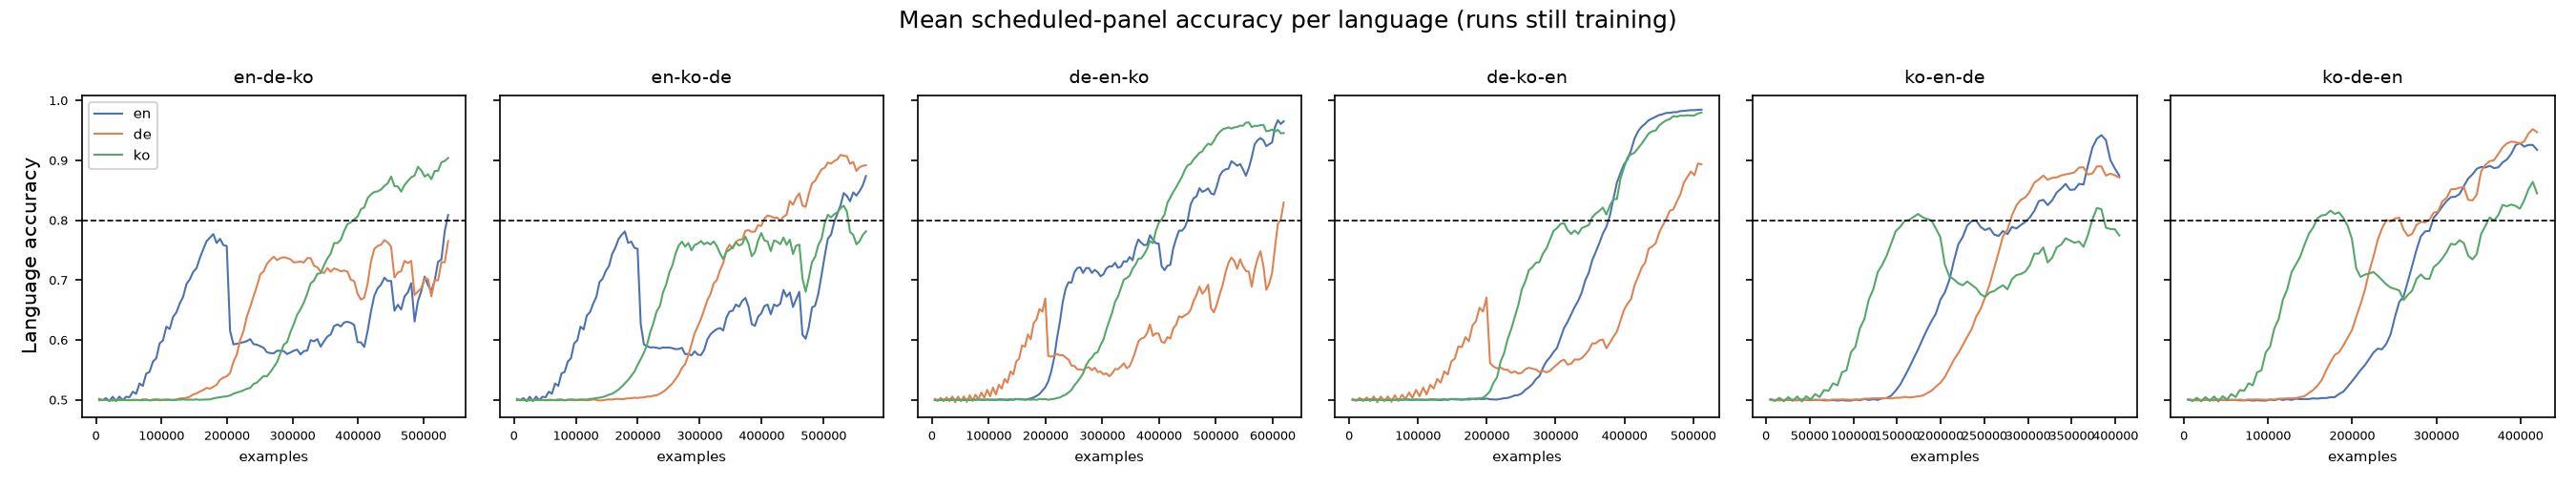
\includegraphics[width=\linewidth]{figures/trajectories-by-order.png}
\caption{Mean scheduled-panel accuracy per language over training, by order, averaged over the runs still training at each point (later points therefore average the slower runs).}
\end{figure}

\begin{figure}[h]
\centering
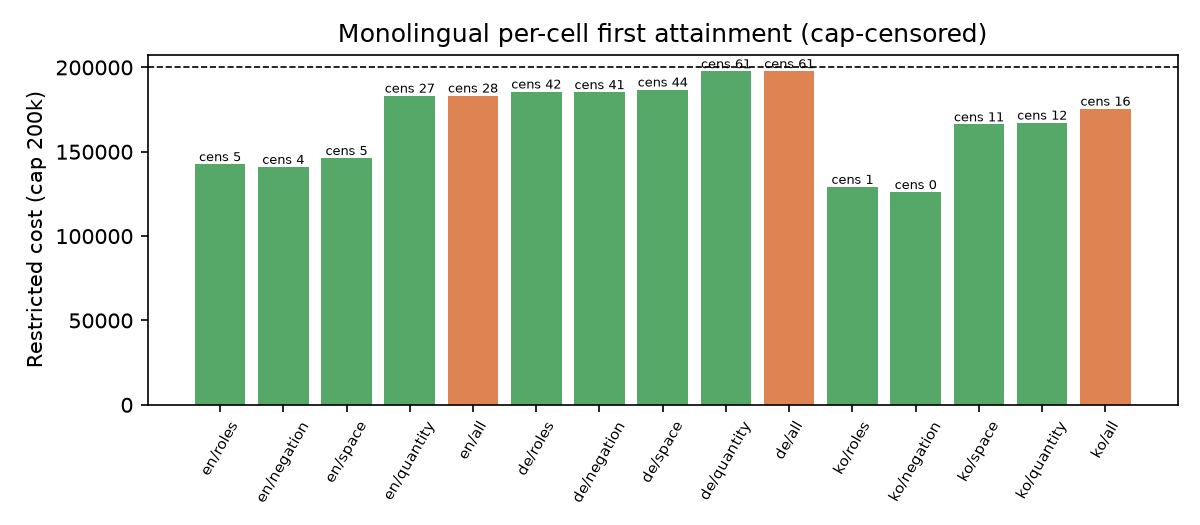
\includegraphics[width=0.85\linewidth]{figures/mono-attainment.png}
\caption{Monolingual restricted mean cost per cell (cap 200{,}000) with censored counts.}
\end{figure}

\section{Simulation design}
\label{app:simulation}

The simulation draws, for each seed block, six order costs from a log-normal or Weibull family with a common coefficient of variation, applies interval censoring at the 5{,}120-example evaluation grid and administrative censoring at the cap with the pilot censoring rate, and imposes the target effect (20\% of the reference mean) on the two contrasts through the reference restricted means calibrated from the pilots. Null scenarios set both effects to zero. Latent correlation between orders was set to zero, the largest grid value not exceeding the lower 2.5\% bootstrap bound of the pilot inter-order correlation. Power rows used 5{,}000 repetitions; null rows were re-run with 50{,}000 repetitions under the amendment of Section~\ref{sec:amendments}, with a correspondence check that the 34 envelope rows are the 17 null distributions crossed with the two targets. The approval quantities are Monte Carlo lower bounds on power and Wilson upper bounds on the family-wise error rate over the envelope. An analytic paired-$t$ cross-check (not used for the decision) gave 21--31 blocks for the first contrast and 10--16 for the second at 80\% power.

\bibliographystyle{elsarticle-harv}
\bibliography{refs}

\end{document}
